\documentclass{article}

\linespread{1.15}
\usepackage[utf8]{inputenc}
\usepackage[left=1.5in,right=1.5in,bottom=1in]{geometry}
\setlength\parindent{0pt}
\setlength{\parskip}{1em}
\setcounter{secnumdepth}{0}
\usepackage{outlines}
\usepackage{graphicx}
\graphicspath{ {imgs} }
\usepackage{hyperref}
\usepackage{color,soul}
\usepackage[normalem]{ulem}

\usepackage[
backend=biber,
style=apa,
citestyle=authoryear,
sorting=nyt,
]{biblatex}
\addbibresource{refs.bib}

\usepackage{comment}
\specialcomment{topicsen}{\begingroup\bfseries\scriptsize}{\endgroup}
%\excludecomment{topicsen}

\newcommand{\alignedmarginpar}[1]{%
        \marginpar{\raggedright\small #1}
    }

\title{Urban Analysis 3}
\author{Carla Hyenne}

\begin{document}

\maketitle

\tableofcontents

\pagebreak

%%%%%%%%%%%%%%%%%%%%%%%%%%%%%%%%%%%%%%%%%%%%%%%%%%%%%%%%%%%%
%											STATEMENT OF PURPOSE
%%%%%%%%%%%%%%%%%%%%%%%%%%%%%%%%%%%%%%%%%%%%%%%%%%%%%%%%%%%%
\section{Statement of Purpose}

Draft 1:

\textbf{I am studying} the (re) conversion of inland, (natural) urban blue spaces into swimmable environments\\
\textbf{because I want to find out} what impact blue spaces can have on a city's social and environmental sustainability\\
\textbf{in order to help my reader understand} the potential that water can have in their city.

Draft 2:

\textbf{I am studying} the (re) conversion of inland, (natural) urban blue spaces into swimmable envrionments\\
\textbf{because I want to find out} how (usable) blue spaces can improve environmental justice in the city\alignedmarginpar{Usable: where people can spend leisure time at and on water.}\\
\textbf{in order to help urban planners understand} the importance of incorporating blue spaces in urban planning and development.

Draft 3:

\textbf{I am studying} the (re) conversion of inland, urban blue spaces into places of leisure at, on or in the water\\ 
\textbf{because I want to find out} the extent to which blue spaces can advance environmental justice\\
\textbf{in order to help my readers understand} the importance of blue space planning policies.

Draft 4:

\textbf{I am studying} the design and use of inland, urban blue space as places of leisure,\\
\textbf{because I want to find out} how the planning \& development of blue spaces shape how they are experienced, and by whom,\\
\textbf{in order to help my readers understand} in what ways blue space can shape environmental justice in the city (or not).


\textit{So what} if we don't know how reconverting blue spaces into swimmable environments can increase environmental justice? If we don't know what the impact that planning for usable blue spaces can have on people, \sout{and the environment}?

What are the \textit{consequences} if the question is not answered?

\begin{outline}
	\1 1. the topic
	\1 2. the condition of the problem that I do not understand $\rightarrow$ question 1
	\1 3. the indirect question, that is wider and more significant than the first one (the condition) $\rightarrow$ question 2
\end{outline}
	
The research is \textit{applied} because it has practical consequences (\cite{booth2003craft}, p. 59)

Notes:

\begin{outline}
	\1 Doesn't include people's health
	\1 I want to focus on public open space --> environmental justice? privatisation of public space taking away opportunities for people to connect to nature and to each other, which is environmentally unjust, and thus open, public blue spaces play an active role in reducing environmental injustice? 
	\1 Environmental justice: the right for people to ---define---
	\1 What about privatisation of space surrounding the water?
	\1 What about where blue spaces are located/renovated? what communities live nearby, have access to it (distance, public transport)?
\end{outline}

%%%%%%%%%%%%%%%%%%%%%%%%%%%%%%%%%%%%%%%%%%%%%%%%%%%%%%%%%%%%
%											PROBLEM STATEMENT AND RQ
%%%%%%%%%%%%%%%%%%%%%%%%%%%%%%%%%%%%%%%%%%%%%%%%%%%%%%%%%%%%
\section{Problem Statement and Research Question}

\textit{To be advancing in your understanding of what you want to know and why that knowledge needs to be produced.
Keep in mind that the aim of the problem statement is to provide a clear reason for your research, and the aim of the research question is to provide a clear direction for your research.}

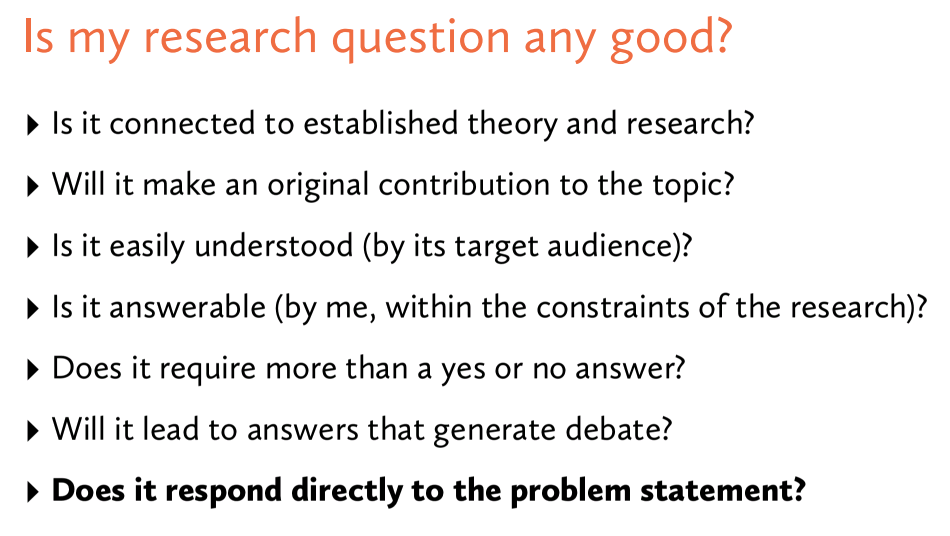
\includegraphics[width=0.75\textwidth]{research_question}

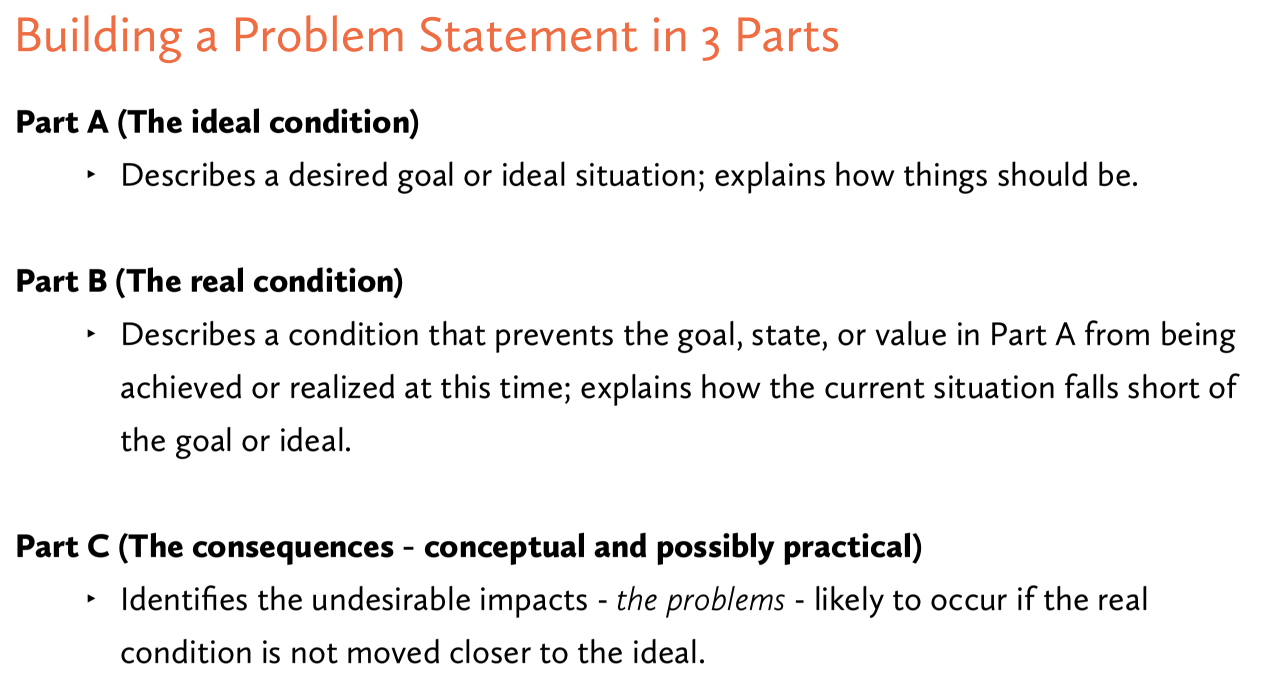
\includegraphics[width=\textwidth]{problem_statement1}

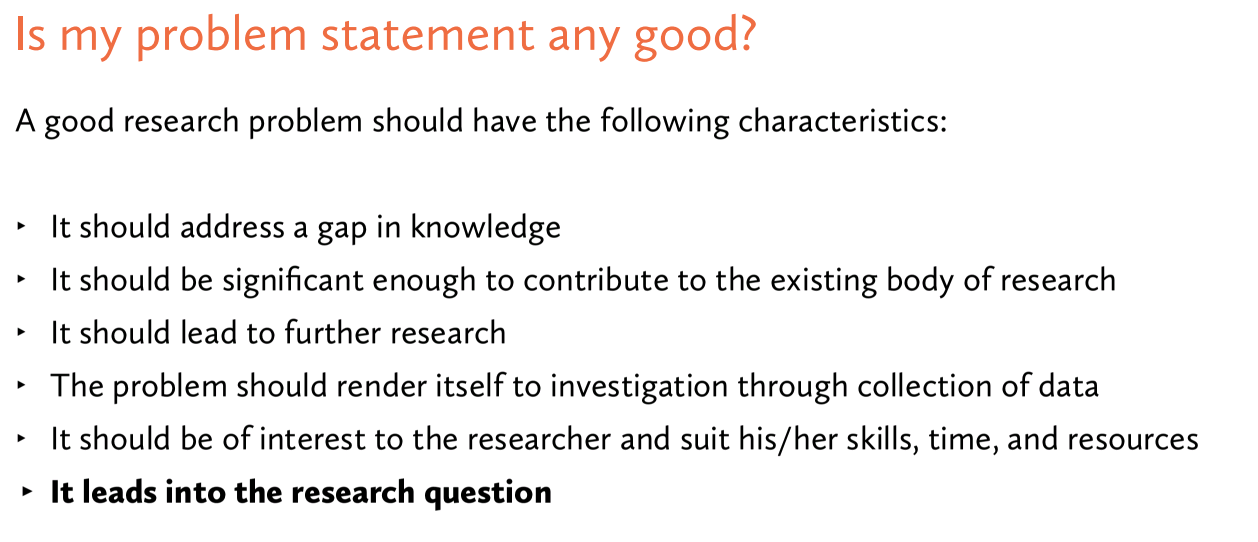
\includegraphics[width=\textwidth]{problem_statement2}

\pagebreak

\subsubsection{Problem statement and Research Question}

Draft 1:

%Environmental justice is a multi-faceted concept which brings together social and environmental concerns. On a general level, it advocates for the equitable access to environmental benefits - and in turn, a share of the environmental burdens.
%especially on deprived population. Thus, blue spaces are an opportunity when it comes to achieving environmental justice.

Interacting both directly or indirectly with blue spaces like rivers, canals, harbours and lakes, has a positive impact on people's mental and physical wellbeing. When public access to blue space is provided, and when the space is well designed, everyone, and especially the more disadvantaged populations, enjoys the benefits.

Urban planning and development influence who uses (blue) space, and how.
If waterfront projects are to contribute to making environmentally just cities, where environmental benefits are equitably shared, then their design has to respond to criteria that account for social and environmental concerns. This includes their location in the city, the built environment, the urban furniture, mobility options, advertising of the space, and more.
Blue spaces should be designed to support a diversity of \textit{users}, and a diversity of \textit{uses}.

Blue spaces which are not designed to be inclusive to people of different ages, genders, cultures, incomes, abilities, etc., reinforce inequalities within the city, and disproportionately affect the lower classes. On the contrary, high-quality blue spaces can contribute to creating cities where diversity, inclusion, accessibility and safety are built-in by design.

Given the above, my research aims to answer the following question: 
what physical and experiential qualities are necessary for a waterfront project to contribute to achieving the goal of environmental justice in the city?

%%%%%%%%%%%%%%%%%%%%%%%%%%%%%%%%%%%%%%%%%%%%%%%%%%%%%%%%%%%%
%											GENERAL IDEAS
%%%%%%%%%%%%%%%%%%%%%%%%%%%%%%%%%%%%%%%%%%%%%%%%%%%%%%%%%%%%
\section{General ideas for the research}

\begin{outline}
	\1 Methodology
		\2 Quantitative: survey data... would need a significant part of the population which will be hard
		\2 Qualitative: contact organisation, NGOs, etc. who work with the blue spaces
		\2 Interview questions:
			\3 Exposure: time of the day/year; 
	\1 Frameworks
		\2 What are the surrounding environments of the blue space? Do certain conditions make the blue space ``better'' (in terms of environmental benefits, usage...), like the facilities, the local environment, the wildlife? (ref. \parencite{garrett2019urban})
		\2 How do we organise people's usage of blue space? For example, the accessibility of the space (incl. distance from home, transport access), indirect/incidental/intentional exposure (ref. \parencite{garrett2019urban})
		\2 Do the type of activities carried out by the users matter, or does simple exposure matter (eg. type of activity, duration of exposure, direct contact with water...)? (ref. \parencite{garrett2019urban})
	\1 Sustainability
		\2 SDG 11: Sustainable cities and communities; Making cities and human settlements inclusive, safe, resilient and sustainable
			\3 11.7 target: ``By 2030, provide universal access to safe, inclusive and accessible, \textbf{green and public spaces}, in particular for women and children, older persons and persons with disabilities''
			\3 11.7 indicator ``Average share of the built-up area of cities that is open space for public use for all, by sex, age and persons with disabilities'' $\rightarrow$ what about blue spaces?
		\2 SDG 3: Good health and wellbeing; Ensure healthy lives and promote well being for all ages
			\3 3.4 Target ``By 2030, reduce by one third premature mortality from non-communicable diseases through prevention and treatment and promote mental health and well-being''
			\3 3.4 Indicator: ``Mortality rate attributed to cardiovascular disease, cancer, diabetes or chronic respiratory disease''
	\1 Urban planning
		\2 How can the learnings on blue spaces be used in urban planning and development frameworks? How can spaces be tailored for their users, in terms of age, or income, for example?
		\2 Is environmental justice inscribed in urban planning/development practices?
		\2 How, or is, the European Union's Green Infrastructure Strategy involved with the city's planning in any way?
		\2 Does the urban planning culture of a city effect how blue spaces are designed or prioritised?
\end{outline}

%%%%%%%%%%%%%%%%%%%%%%%%%%%%%%%%%%%%%%%%%%%%%%%%%%%%%%%%%%%%
%											CONCEPTS
%%%%%%%%%%%%%%%%%%%%%%%%%%%%%%%%%%%%%%%%%%%%%%%%%%%%%%%%%%%%

\subsection{Environmental Justice}

\begin{outline}
	\1 A multi-dimensional concept
	\1 A term originating from the US, and North American research focuses on the intersection of the environment with race. There are other dimensions than race that can be explored, like age, gender, income, physical or mental abilities...
	\1 Three dimensions of justice: distributive/distributional, procedural/participatory, and interactional/recognition \parencite{kronenberg2020environmental}
\end{outline}

\section{Frameworks}

\begin{outline}
	\1 Characteristics of a blue space: what should it have, or not have, in order to be pleasant, safe, used? \parencite{}
\end{outline}




%%%%%%%%%%%%%%%%%%%%%%%%%%%%%%%%%%%%%%%%%%%%%%%%%%%%%%%%%%%%
%											READINGS
%%%%%%%%%%%%%%%%%%%%%%%%%%%%%%%%%%%%%%%%%%%%%%%%%%%%%%%%%%%%
\section{Readings}

\subsubsection{Garrett et al., \textit{Urban blue spaces and health and wellbeing in Hong Kong: Results from a survey of older adults}, 2019} \parencite{garrett2019urban}

\begin{outline}
	\1 What are the potential health benefits of being near to, seeing, using blue spaces? The study looks are the perceived well-being of elderly in Hong-Kong
	\1 The benefits of green spaces in urban environments are known. Dense, stressful, polluted urban environments can cause physical and mental illnesses, and green spaces can help reduce these symptoms. Three main ways in which green and health are linked (according to Markevych et al., (p. 100)):
		\2 ``Reducing environmental harms (eg. mitigating noise pollution)'' $\rightarrow$ environment
		\2 ``Supporting emotion regulation and the restoration of depleted cognitive capacities (eg. through stress alleviation)'' $\rightarrow$ social
		\2 ``Building capacities (eg. through supporting physical activity)'' $\rightarrow$ social
	\1 Blue spaces provide similar benefits, like reducing stress, heart diseases, making people more physically active, etc. But to what extent do you need to frequent the blue spaces to gain these benefits? How much blue/green space is required in order to get the benefits
	\1 Three research questions: (p. 101)
		\2 ``To what extent is self-reported general health and wellbeing in Hong Kong related to an individuals exposure to the city's blue spaces?''
		\2 ``Which environmental factors predict blue space visit frequency in Hong Kong?''. They looked at the safety, presence of wildlife, clean/free from litter, and good facilities like footpaths or toilets
		\2 ``Are some visit and environmental characteristics associated with better short-term recalled wellbeing outcomes?''
	\1 The conclusion, indirect and intentional exposure were associated with good health and high level of wellbeing; good facilities and wildlife are related to intentional usage; safety and wildlife are related to higher levels of wellbeing and g when visiting the blue space; visible blue space from home is related to better perceived health; those who regularly visit/see from home blue spaces are more likely to have good mental health and good general health.
	
	\1 $\Rightarrow$ This paper analyses the perceived health benefits that blue spaces can have on the population (it focuses on elderly residents). It defines three categories of blue space exposure: indirect (view from home), incidental (on commute route), and intentional (purposeful visit), and addresses different factors that could influence people's perception and use of the blue space, like safety, cleanliness, facilities, accessibility. They find a positive relation between blue space and overall wellbeing, including good health and good mental health.
	It recognises the particularities of Hong Kong: it is surrounded by water, has high quality and safe public space, a fantastic public transit system (which makes it easy for people to reach blue spaces if they don't live nearby). I think it is necessary to acknowledge these particularities in a city, because they can influence how people interact with blue (or green) spaces.
	
	Why is it relevant to me? It provides a categorisation of blue space usage, and a framework for analysing the benefits and quality of blue spaces. It focuses on the effect that blue spaces have on the physical wellbeing of people, and this falls under social sustainability. 
\end{outline}

\subsubsection{Gascon et al., \textit{Outdoor blue spaces, human health and well-being: A systematic review of quantitative studies}, 2017} \parencite{gascon2017outdoor}

\begin{outline}
	\1 Summarises the quantitative evidence from existing research on the positive effects of blue spaces on people's health, and concludes that there is a correlation between blue space exposure and benefits in mental health and in wellbeing. Says there is too few and too much heterogeneity in the studies
	\1 There are claims of the positive effect of blue space on people's health and wellbeing, either by being \textbf{proximally or distally/virtually} (being in, on or near/being able to see, hear or sense water). The effects of blue spaces could be similar to that of green spaces, which include ``stress reduction, increased physical activity, promotion of positive social contacts, increased place attachement and the reduction of extreme temperatures'' (p. 1212)
	\1 Differentiates outdoor blue space type into inland (rivers, lakes, ponds, streams, rivulets, wetlands, freshwaters) and non-inland (coast, beach, salt waters)
	
	\1 $\Rightarrow$ This paper reviews quantitative studies on blue space and associated health benefits. It reports the type of blue space, the environment of the blue space, and how the health outcomes were evaluated.
	What I found useful was the differentiation between inland and non-inland spaces, which I will use in my research. I also realised I don't want to focus specifically on the relation of blue space to human health (eg. general health, mental health and wellbeing, physical activity, other morbidities) because there is already good research in this area, especially in Europe. I still want to focus on the social aspect of blue spaces, but perhaps more on blue spaces as open, public and free spaces. Also, quantitative research will be hard because I don't think I would be able to reach enough participants (I assume in the scale of hundreds?) in both case studies
\end{outline}

\subsubsection{Raymond et al., \textit{Integrating multiple elements of environmental justice into urban blue space planning using public participation geographic information systems}} \parencite{raymond2016integrating}

\begin{outline}
	\1 Uses PPGIS (Public Participation Geographic Information System) method for ``spatially identifying and assessing multiple elements of environmental justice in urban blue space''. Using Finland as a case study, it looks for:
		\2 ``Diversity and spatial distribution of clusters base don the activities undertaken in urban blue space''. A cluster is an area defined by the type of activity carried out there
		\2 ``Diversity of users in each cluster, representing a composite measure of income, age and family income'', also race, gendre, disabilities. How facilities and services influence who uses the space
		\2 ``Extent of perceived problems and unpleasant experiences in each cluster'' 

	\1 \hl{Environmental justice}: a principle that claims that all people have a right to be protected from environmental pollution, and live in a clean and healthy environment. 
		\2  PPGIS enables urban planning to tailor blue spaces to specific types of activities and users. It is used within the context of environmental justice, because it helps analyse user diversity (the mix of users) and perceived problems and unpleasant experience (PPUE, the perceived negative qualities of a place). PPGIS can help analyse how ``different elements of environmental justice are spatially distributed across the landscape. Understanding environmental justice from multiple perspectives is crucial to ensuring that urban settings are designed in ways that contribute to a range of place-based experiences, including social interactions between diverse user groups, as well as provide possibilities for connection to nature. '' (p. 199)
		\2 Environmental justice resonates with SDG 11 to ``provide universal access to safe, inclusive and accessible, green and public spaces''
		\2 Privatisation of urban space is taking away opportunities for people to connect with each other, and with nature
		\2 \textbf{Multiplicity as a principle in urban inclusion} may create conflict between different user types and PPUE, based for example on the types of activities offered, and can lead to feelings of exclusion, discomfort or fear\alignedmarginpar{Inclusivity in public space\\Right to blue space}
	\1 Helsinki and surrounding regions as case study: the context is that Helsinki residents are never more than 10km away from the shore
		\2 Survey asked participants about PPUE (encompasses cost, inclusivity, facilities, environment, safety...), usage based on time of year, activity, socio-demographic features (age, income, ethnicity, family situation...)
		\2 Income level was a strong determinator of accessibility
	\1 Environmental justice is multidimensional: the paper takes into account user diversity, activity diversity, and PPUE
		\2 Using four-quadrant framework for combining user diversity and activity diversity (high/low user diversity, high/low activity diversity matrix), they classify areas (``clusters''), for eg. Helsinki shorelines are mostly hi user/lo activity diversity, and lo user/hi activity diversity ]
		\2 By classifying areas into these quarters, they could see what type of blue space existed (in terms of users and activities), and find some characteristics of the quarters (eg. more nature activities in one area, maybe because of the environment?)
	\1 Most cited PPUE was ``certain group of people or use method bothers me'', ``the environment is littered or not cared for'', ``the water quality is poor'', ``the location is crowded''
	\1 $\Rightarrow$ This paper focuses on environmental justice which I think is a great term to help frame my research interest, because it incorporates principles like sustainability, inclusivity, and right to open blue spaces. The paper looks at the diversity of users, diversity of activities, and the PPUE (perceived problems and unpleasant experience) of the blue spaces, to demonstrate the multidimensionality of environmental justice. It also made me wonder whether I should focus on a certain socio-demographic group (by age, income levels, gender, ethnicity, etc.), and  how that group is affected by the presence, uses, and/or design of blue spaces, or lack thereof. 

\end{outline}

\subsubsection{van den Bogerd et al., \textit{Urban blue space renovation and local resident and visitor well-being: A case study from Plymouth, UK}, 2021}

\parencite{van2021urban}

\begin{outline}
	\1 Access to ``attractive, safe and inclusive blue spaces'' heightens people's psychological wellbeing, and especially that of those living in \hl{deprived urban areas}
	\1 The first study to evaluate the impact of small scale interventions (where the built environment was altered) in a deprived urban area, on the psychological wellbeing of the residents/users. The well being of the residents and visitors was assessed (by self reporting) before and after the intervention. Community was involved in the project
		\2 BlueHealth did ``urban blue acupuncture'' interventions, to evaluate the extent to which small scale/modest intervention can positively impact mental health
		\2 Hypothesis was three fold (p. 3), importance of site quality, feelings of personal safety, and community belonging
		\2 The renovation included: a theatre with seating facing the water, removing parking on the access path, renovating the ``slipway'' (access path), improving the playground (p. 3, 2.1)
		\2 They emphasise the importance of involving the residents in the renovation, and acknowledge that doing so makes it hard to understand whether the increase in wellbeing is due to the renovated infrastructure, or the experience of being involved in a community project
	\1 Result was a greater sense of wellbeing due to a feeling of community belonging; and a greater sense of life satisfaction due to ``greater satisfaction with personal safety and community belonging''
	\1 Challenges in upscaling/upgrading green and blue spaces
		\2 Are people who live near green and blue spaces healthier and happier because of their proximity to the spaces, or is it that people with greater health and happiness happen to live near green and blue spaces because they can afford to and choose to?
		\2 Do the interventions lead to gentrification, causing wealthier and healthier populations to move in?
		\2 $\rightarrow$ this study calls for more research in areas where the population is stable: eg. areas with a large number of social housing which will stay social and where wealthier populations will not move in
	\1 Potential benefits of blue spaces in deprived areas
		\2 Populations in deprived areas/low socio-economic status have poorer mental and physical health, and 
		\2 Visits to coastal blue spaces is more equitable across socio-economic groups, compared to woodland (p. 2, 1.1)
	\1 Potential mechanisms
		\2 Better environment quality leads to better health benefits; in particular, (good) facilities, improved access to riverbank, presence of wildlife. Eg. riverbank in Barcelona
		\2 Blue space renovation leads to increased feelings of safety, which in turn positively influences mental health; qualitative investigation on blue spaces shows that feelings of safety greatly increases the use of blue spaces (p. 3, 1.2) 
		\2 Community belonging, a sense of community and social cohesion ``mediate'' relation between green space and mental wellbeing
\end{outline}

\subsubsection{Wessells, \textit{Urban Blue Space and ``The Project of the Century'': Doing Justice on the Seattle Waterfront and for Local Residents}, 2014}

\parencite{wessells2014urban}

\begin{outline}
	\1 Brings together four perspectives of ``doing justice'' in the waterfront area: \hl{economic justice, environmental justice, social justice, tribal justice}. Each dimension comes with a its own challenges. The paper defines the scale of blue spaces as local and regional, and asks how waterfront revitalisation projects can address public trust, public spaces as common goods, and right to the city
		\2 This demonstrates that the challenge is to ``construct a place that works to counter established patterns of local and regional injustice'' (p. 764)
		\2 Blue space is conceived as a ``shared public and environmental good'', and is as important as green space, ``constituting their own species of urban space, whose urban political ecology is essential to the sustainable development of cities and urban regions'' (p. 765)
		\2 Seattle branded as a progressive and inclusionary place but still follows the pattern of high-growth, creative class, inequitable cities (p. 776)
		\2 ``In order to do justice on the waterfront, it may be more effective and efficient to identify the dynamics and outcomes that reinforce patterns of privilege and discrimination and proactively convene the leaders, groups and activists most impacted by such patterns and best poised to devise alternative paths forward'' (p. 776)
	\1 Physical setting and built environment
		\2 Routes and connections: cars present a physical barrier between the city and waterfront, there are only disjointed and no unified pedestrian connections; haphazard parking; 
	\1 Blue spaces as sustainable spaces: sustainability encompasses ``economic, environmental, social and cultural'' dimensions and blue spaces extends to all of them
		\2 Blue spaces as social spaces: ``of gathering, labour, economic exchange, recreation, subsistence fishing, cultural tradition and journey-making'' (p. 766)
		\2 Blue spaces as ecological spaces: ``of watershed catchment, primary productivity, near-shore habitat, species migration and environmental degradation'' 
		\2 Blue space is \textbf{permeable}, and isn't only the border of water with land (the waterfront). It encompasses the social (\hl{shared public space}) and the environmental
	\1 Scale of blue spaces: local and regional governance; they need to be managed
		\2 ``Is the ``public trust'' of the urban waterway as an environmental resource bing protected as a \hl{common good}? Is the ``\hl{right to the city}'' of urban residents being enabled through waterfront land uses?''
		\2 Tendency to favour ``established economic interests'' over grass-roots, community stakeholders
	\1 Economic justice: entrepreneurial/neoliberal context makes it harder for local, small businesses and projects to take root; there's a need to protect affordable housing, empower local entrepreneurs, support minimum wage standards, divert from revenue intensive ideology
	\1 Environmental justice: tendency for polluting industries to be located near \hl{low income/minority neighbourhoods}, and green revitalisation projects tend to be close to upper middle class neighbourhoods
		\2 To address \hl{environmental justice}, the waterfront should focus on ``the relative accessibility of the waterfront site to different populations; second, the relationship between the central waterfront and public investment in other Seattle shoreline sites; and finally, the quality of the environmental remediation that takes place'' (p. 771) $\rightarrow$ diversity of users; routes and connections;
		\2 Accessibility: site design, physical infrastructure, and the activities/behaviours they support; proximity by foot, bike, public transport, car; 
		\2 Considering the waterfront in a relationship to other waterfronts; not privileging already privileged areas (socio-economic situation) to the detriment or the ignorance of other spaces, which have more dire needs like making the space safe to use 
	\1 Social justice: concern with social difference and inclusive democracy, highlights the concentration of social power amongst those with highest socio-economic status/the majority
		\2 \hl{Social production of space}: a space is socially constructed and inhabited, ``it is through the social practices that become normalised in urban space, that the ``right to the city'' is exercised, produced and sustained'' (p. 773) $\rightarrow$ even if a space is physically accessible and public, those whose social practices and behaviours are different than that of the majority who use the space, will not feel welcome
		\2 \hl{Social practices of exclusion}: increasing privatisation of public space, encouraging consumption, spending money to fit in socially, excluding people based on socio-economic class, social relations are less public and thus less diversity of activities in the public realm; segregation by socio-economic means; women experiencing space different than men, feeling threatened
	\1 Tribal justice
\end{outline}

\subsubsection{}

\begin{outline}
	\1 Brief history of environmental justice in the US
\end{outline}

%%%%%%%%%%%%%%%%%%%%%%%%%%%%%%%%%%%%%%%%%%%%%%%%%%%%%%%%%%%%
%											OTHER MATERIAL
%%%%%%%%%%%%%%%%%%%%%%%%%%%%%%%%%%%%%%%%%%%%%%%%%%%%%%%%%%%%

\subsection{Material (not papers)}

\subsubsection{Blue Health}

\url{https://bluehealth2020.eu/}

\begin{outline}
	\1 Focuses on impact of blue spaces on climate and human health
\end{outline}

\subsubsection{Copenhagen Waterfront Design Catalogue}

\parencite{copenhagenwaterfront}

\begin{outline}
	\1 Proposes 6 sections ``as ideas for the design of waterfronts, promenades/esplanades, activities and areas for gathering at and on the water'' (purpose). Each section has ideas for development. They are:
		\2 Waterfronts: ideas for infrastructure to make the waterfront itself more accessible (stairs, edges, seating areas...)
		\2 Access to the water: direct access for swimming/boating/lounging/fishing/other activities
		\2 Public waterfront areas: creating a pleasurable, fun, safe, inclusive environment around the water
		\2 Routes and connections: interconnectedness of the harbour, with soft-mobility routes (foot and bike paths)
		\2 Temporary use: ephemeral infrastructure while the waterfront area is undergoing development, to encourage visits
		\2 Activities: making a wide range of activities in, on and around the water available, and the infrastructure to support them (eg. stage, showers,...)
\end{outline}

%%%%%%%%%%%%%%%%%%%%%%%%%%%%%%%%%%%%%%%%%%%%%%%%%%%%%%%%%%%%
%											ASSIGNMENTS
%%%%%%%%%%%%%%%%%%%%%%%%%%%%%%%%%%%%%%%%%%%%%%%%%%%%%%%%%%%%

\pagebreak

\begin{flushright}
Carla Hyenne\\
Urban Analysis 3
\end{flushright}

\subsection{Problem Statement and Research Question}

Interacting directly or indirectly with blue spaces like rivers, canals, harbours and lakes, has a positive impact on people's mental and physical wellbeing. 
When public access to blue space is provided, and when the space is well designed, everyone enjoys the benefits.
If waterfront projects are to contribute to making environmentally just cities, %where environmental benefits are equitably shared, then 
their design has to respond to subjective criteria that account for social and environmental concerns. \\
Urban planning and development influence who uses (blue) space, and how. As such, blue spaces should be designed to support a diversity of \textit{users}, and a diversity of \textit{uses}. \\
Blue spaces which are not designed to be inclusive to people of different ages, genders, cultures, incomes, abilities, etc., reinforce inequalities within the city, and disproportionately affect the lower classes. 
%On the contrary, high-quality blue spaces can contribute to creating cities where diversity, inclusion, accessibility and safety are built-in by design.
% and especially the more disadvantaged populations.
%This includes their location in the city, the built environment, the urban furniture, mobility options, advertising of the space, and more.

Given the above, my research aims to answer the following question: 
what physical and experiential qualities are necessary for a waterfront project to contribute to achieving the goal of environmental justice in the city?

Ideal: 

Reality:

Consequences:


\pagebreak

\printbibliography

\end{document}

\subsubsection{}

\begin{outline}
	\1
\end{outline}

